\documentclass{article}

\usepackage[utf8]{inputenc}
\usepackage{polski}

\usepackage[simplified]{pgf-umlcd}
\begin{document}
    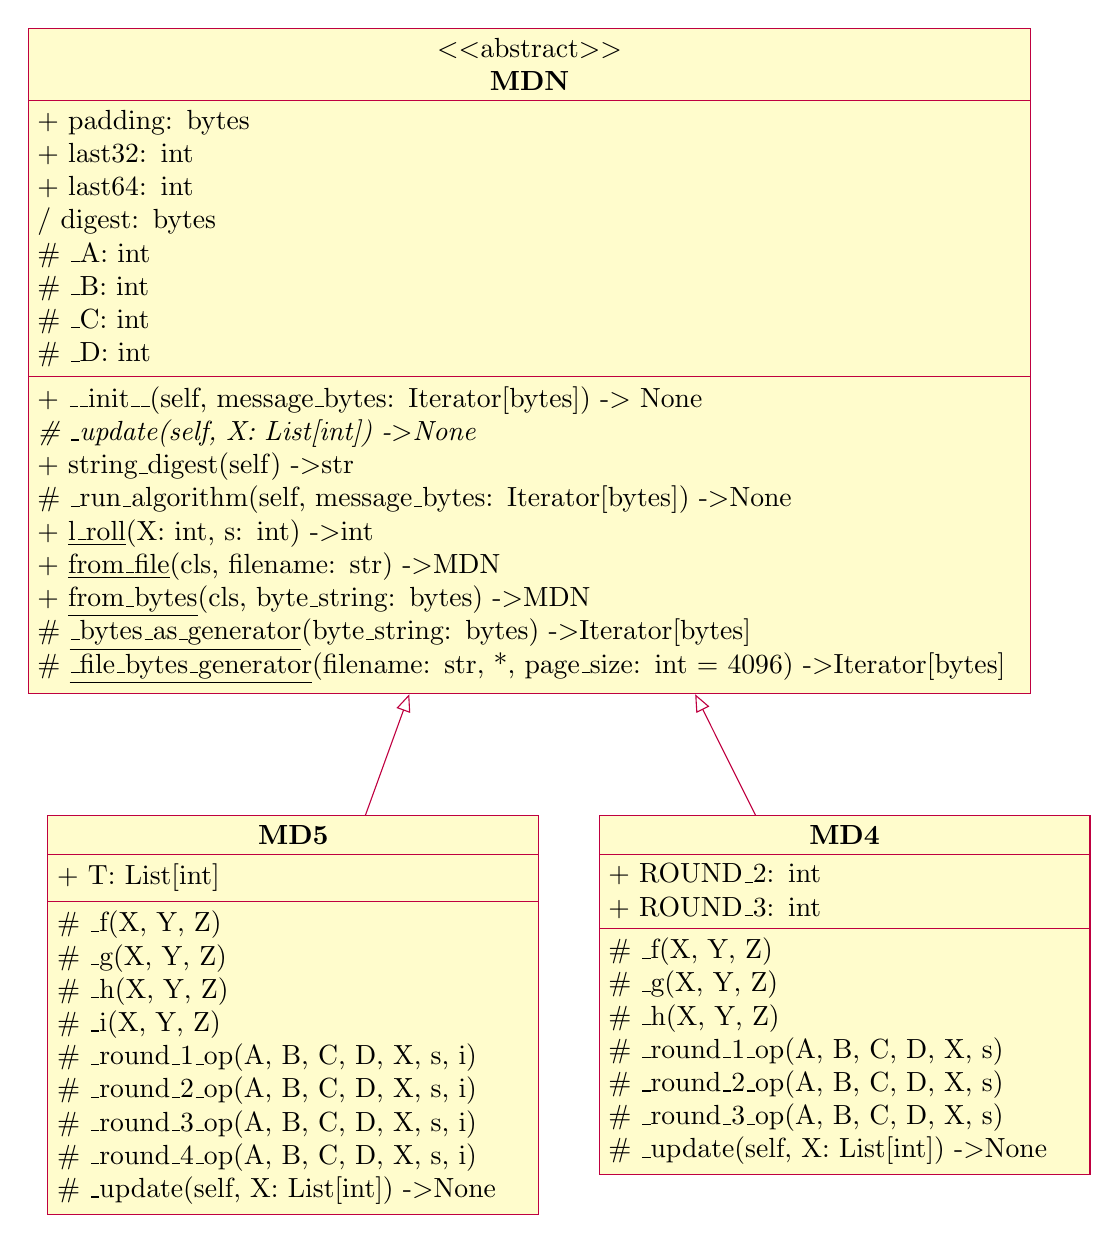
\begin{tikzpicture}
        \begin{abstractclass}[text width=12.5cm]{MDN}{0,10}
            % class constants
            \attribute{+ padding: bytes}
            \attribute{+ last32: int}
            \attribute{+ last64: int}
            % object attributes
            \attribute{/ digest: bytes}
%digest(self)
            \attribute{\# \textunderscore A: int}
            \attribute{\# \textunderscore B: int}
            \attribute{\# \textunderscore C: int}
            \attribute{\# \textunderscore D: int}

            % init
            \operation{+ \textunderscore\textunderscore init\textunderscore\textunderscore (self, message\textunderscore bytes: Iterator[bytes]) -\textgreater\ None }
            % abstract method
            \operation[0]{\# \textunderscore update(self, X: List[int]) -\textgreater None}

            % concrete methods
            \operation{+ string\textunderscore digest(self) -\textgreater str}
            \operation{\# \textunderscore run\textunderscore algorithm(self, message\textunderscore bytes: Iterator[bytes]) -\textgreater None}
            \operation{+ \underline{l\textunderscore roll}(X: int, s: int) -\textgreater int}

            \operation{+ \underline{from\textunderscore file}(cls, filename: str) -\textgreater MDN}
            \operation{+ \underline{from\textunderscore bytes}(cls, byte\textunderscore string: bytes) -\textgreater MDN}

            \operation{\# \underline{\textunderscore bytes\textunderscore as\textunderscore generator}(byte\textunderscore string: bytes) -\textgreater Iterator[bytes]}
            \operation{\# \underline{\textunderscore file\textunderscore bytes\textunderscore generator}(filename: str, *, page\textunderscore size: int = 4096) -\textgreater Iterator[bytes]}
        \end{abstractclass}

        \begin{class}[text width=6cm]{MD4}{4,0}
            \inherit{MDN}
            \attribute{+ ROUND\textunderscore2: int}
            \attribute{+ ROUND\textunderscore3: int}

            \operation{\# \textunderscore f(X, Y, Z)}
            \operation{\# \textunderscore g(X, Y, Z)}
            \operation{\# \textunderscore h(X, Y, Z)}
            \operation{\# \textunderscore round\textunderscore 1\textunderscore op(A, B, C, D, X, s)}
            \operation{\# \textunderscore round\textunderscore 2\textunderscore op(A, B, C, D, X, s)}
            \operation{\# \textunderscore round\textunderscore 3\textunderscore op(A, B, C, D, X, s)}

            \operation{\# \textunderscore update(self, X: List[int]) -\textgreater None}
        \end{class}
        \begin{class}[text width=6cm]{MD5}{-3,0}
            \inherit{MDN}
            \attribute{+ T: List[int]}

            \operation{\# \textunderscore f(X, Y, Z)}
            \operation{\# \textunderscore g(X, Y, Z)}
            \operation{\# \textunderscore h(X, Y, Z)}
            \operation{\# \textunderscore i(X, Y, Z)}
            \operation{\# \textunderscore round\textunderscore 1\textunderscore op(A, B, C, D, X, s, i)}
            \operation{\# \textunderscore round\textunderscore 2\textunderscore op(A, B, C, D, X, s, i)}
            \operation{\# \textunderscore round\textunderscore 3\textunderscore op(A, B, C, D, X, s, i)}
            \operation{\# \textunderscore round\textunderscore 4\textunderscore op(A, B, C, D, X, s, i)}
            \operation{\# \textunderscore update(self, X: List[int]) -\textgreater None}
        \end{class}
    \end{tikzpicture}
\end{document}
